% This example is meant to be compiled with lualatex or xelatex
% The theme itself also supports pdflatex
\PassOptionsToPackage{unicode}{hyperref}
\documentclass[aspectratio=1610, 9pt, xcolor=dvipsnames]{beamer}
\usepackage[absolute,overlay]{textpos}
\usepackage{graphicx,caption}
\parskip0pt
% Load packages you need here
\usepackage{polyglossia}
\setmainlanguage{german}

\usepackage{csquotes}

\usepackage{tikz}

\usepackage{subfig}

\usepackage[export]{adjustbox}

\usepackage{amsmath}
\usepackage{amssymb}
\usepackage{mathtools}
\usepackage{unicode-math}
\usepackage{xfrac}

\usepackage{environ}

\usepackage{hyperref}
\usepackage{bookmark}
\usepackage{graphicx}
\usepackage{wrapfig}

\usepackage{booktabs}

\usepackage{multicol}

\usepackage{relsize}

\usepackage[dvipsnames]{xcolor}

\usepackage{bm}

\usepackage{empheq}
\newcommand*\widefbox[1]{\fbox{\hspace{2em}#1\hspace{2em}}}

\makeatletter
\newcommand{\Pause}[1][]{\unless\ifmeasuring@\relax
\pause[#1]%
\fi}
\makeatother

\usepackage[
locale=DE,
separate-uncertainty=true, % Immer Unsicherheit mit ±
per-mode=symbol-or-fraction, % m/s im Text, sonst \frac
% alternativ:
% per-mode=reciprocal, % m s^{-1}
% output-decimal-marker=., % . statt , für Dezimalzahlen
]{siunitx}

% load the theme after all packages

\usetheme[
  showtotalframes, % show total number of frames in the footline
]{tudo}

% Put settings here, like
\unimathsetup{
  math-style=ISO,
  bold-style=ISO,
  nabla=upright,
  partial=upright,
  mathrm=sym,
}

\DeclarePairedDelimiter{\bra}{\langle}{\rvert}
\DeclarePairedDelimiter{\ket}{\lvert}{\rangle}
\DeclarePairedDelimiterX{\braket}[2]{\langle}{\rangle}{
#1 \delimsize| #2
}

\newenvironment<>{varblock}[2][.9\textwidth]{%
  \setlength{\textwidth}{#1}
  \begin{actionenv}#3%
    \def\insertblocktitle{#2}%
    \par%
    \usebeamertemplate{block begin}}
  {\par%
    \usebeamertemplate{block end}%
  \end{actionenv}}


\NewEnviron{myequation}{%
  \begin{equation*}
  \scalebox{1.5}{$\BODY$}
  \end{equation*}
}

%----------------------------------------
%Align Equations to LEFT MARGIN (use \mathleft then \mathcenter)
\makeatletter
\newcommand{\mathleft}{\@fleqntrue\@mathmargin0pt}
\newcommand{\mathcenter}{\@fleqnfalse}
\makeatother
%----------------------------------------

\title{Quantum annealing und Logistik}
\author[Y.~Kind]{Yanick Kind}
\institute[]{Fakultät Physik}
\date{12. Juli 2023}


\begin{document}

\maketitle

\begin{frame}{Übersicht}
  \begin{columns}
    \column{0.4\linewidth}
    \setlength{\parskip}{4ex}
    \tableofcontents
    \column{0.6\linewidth}
    \vspace*{1cm}
    \centering
    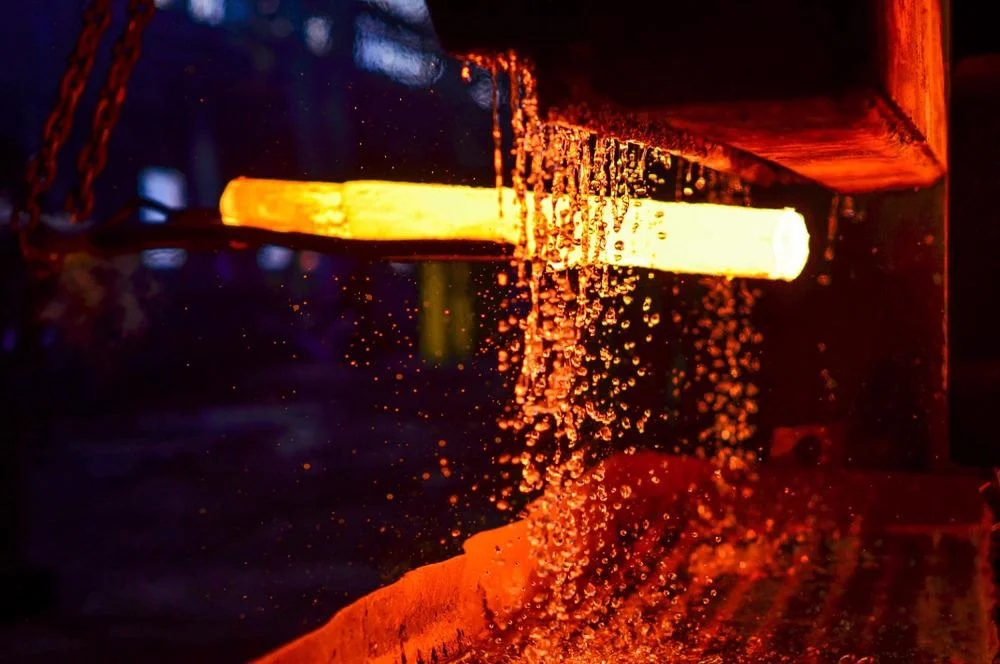
\includegraphics[width = \textwidth]{Plots/annealing_front.png}
    \hspace*{12pt}\hbox{\scriptsize {\footnotesize\itshape \href{https://www.azom.com/article.aspx?ArticleID=20342}{azom.com}}}
  \end{columns}
\end{frame}

\section{Einleitung}

\begin{frame}{Traveling Salesman problem}
  \begin{itemize}
    \item klassisches kombinatorische Optimierungsproblem
    \item Beispiel: Ein Lieferwagen hat $n$ Lieferorte
    \begin{itemize}
      \item[\textrightarrow] $(n-1)!$ verschiedene Routen
    \end{itemize}
    \item NP-hard
    \begin{itemize}
      \item[\textrightarrow] skaliert nicht polynomiell sondern \textbf{exponentiell} mit Systemgröße
    \end{itemize}
    \item Globales Optimum mittels numerischen Lösungsverfahren finden, ist extrem aufwändig
    \item Local search Algorithmen als heuristische Näherungsverfahren nutzen
  \end{itemize}  
\end{frame}

\begin{frame}{Motivation}
  \begin{columns}
    \column{0.3\linewidth}
       \centering
       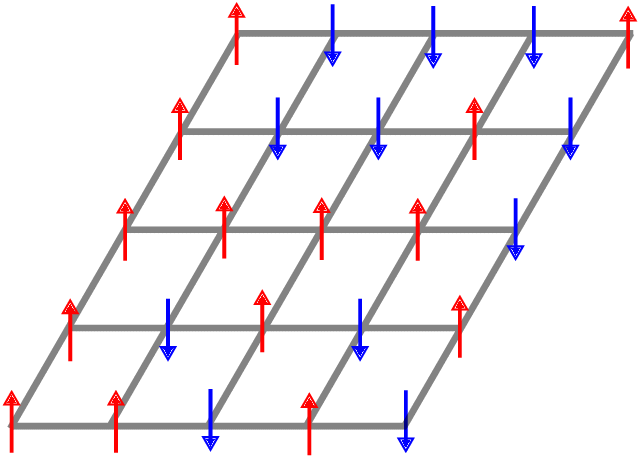
\includegraphics[width = 0.95\textwidth]{Plots/Ising_Modell_2d.png}
       \hspace*{12pt}\hbox{\scriptsize {\footnotesize\itshape \href{https://www.researchgate.net/publication/321920877_Thermalisation_and_Relaxation_of_Quantum_Systems}{Sascha Wald, Thermalisation and Relaxation of Quantum Systems (2017)}}}
       \\ 
       \vspace*{1cm}
       \scalebox{3}{$E$}
    \column{0.2 \linewidth}
    \centering  
      \vspace*{2.2cm}
      \scalebox{4}{$\stackrel{?}{\to}$}
    \column{0.3\linewidth}
      \centering
      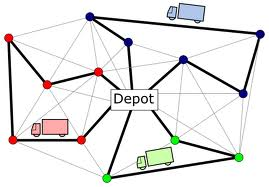
\includegraphics[width = 0.95 \textwidth]{Plots/vehicle_routing_problem.jpg}
      \hspace*{12pt}\hbox{\scriptsize {\footnotesize\itshape \href{https://www.r-bloggers.com/2010/11/any-r-packages-to-solve-vehicle-routing-problem/}{r-bloggers.com}}}
      \\
      \vspace*{1cm}
      \scalebox{3}{$f$}
 \end{columns}
\end{frame}

\begin{frame}{Motivation}
  \centering
  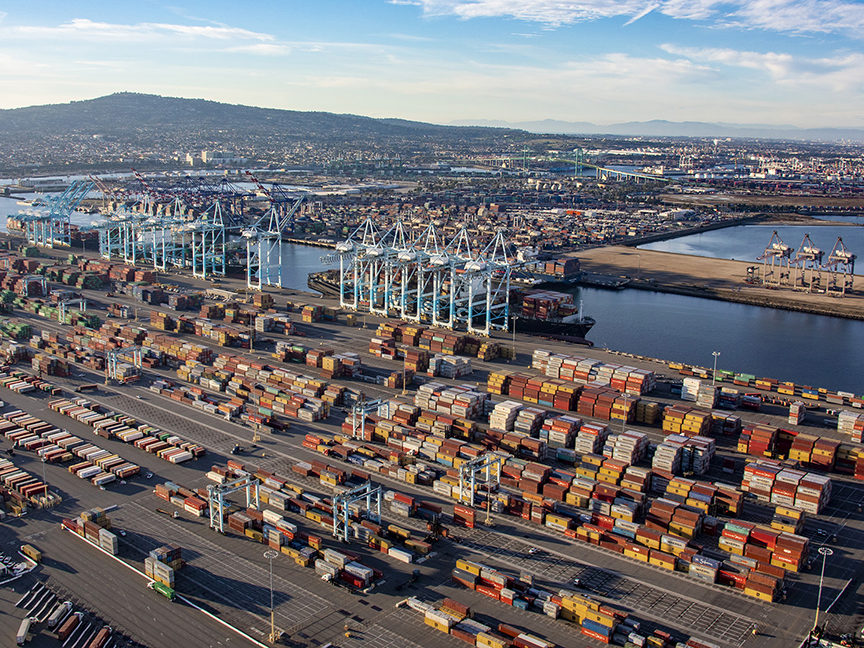
\includegraphics[width = 0.6\textwidth]{Plots/LA.jpg}
\end{frame}

\section{Simulated und quantum annealing}

\begin{frame}{Simulated annealing}
  \begin{itemize}
    \item in Analogie zu auskühlenden Metallen
    \begin{itemize}
      \item schneller auskühlen \textrightarrow suboptimalerer Zustand (amorph)
      \item langsamer auskühlen \textrightarrow optimalerer Zustand (kristallin)
    \end{itemize}
    \item nutzt thermische Fluktuationen, um lokalen Minima zu entkommen
    \item Wahrscheinlichkeit $P_i$ folgen Mastergleichung $\frac{dP_i}{dt} = \sum_j L_{ij} P_j$
    \begin{itemize}
      \item        $L_{ij} = 
      \begin{cases}
        \left [ 1 + \text{exp}((E_i -E_j) / T_t) \right ]^{-1}  & \, \text{einzelne Spin Differenz} \\
        - \sum_{k \neq i} L_{ki}                                & \, i = j \\
        0                                                       & \, \text{sonst}
      \end{cases}
    $
    \end{itemize}
  \end{itemize}
  \begin{textblock*}{6cm}(9.2cm,3cm) % {block width} (coords)
  
\includegraphics[width = 6.5cm, angle=270,origin=c]{Plots/slow_fast_SA.png}
  %\hspace*{12pt}\hbox{\scriptsize {\footnotesize\itshape \href{https://en.wikipedia.org/wiki/}{Cyp, wikipedia.org}}}
  \end{textblock*}    
\end{frame}

\begin{frame}{simulated annealing}
  Bild um die Übergangselemente zu erläutern in Inkscape selber machen
\end{frame}

\begin{frame}{Quantum Annealing}
  \begin{itemize}
    \begin{textblock*}{5cm}(10.4cm, 2.05cm) % {block width} (coords)
      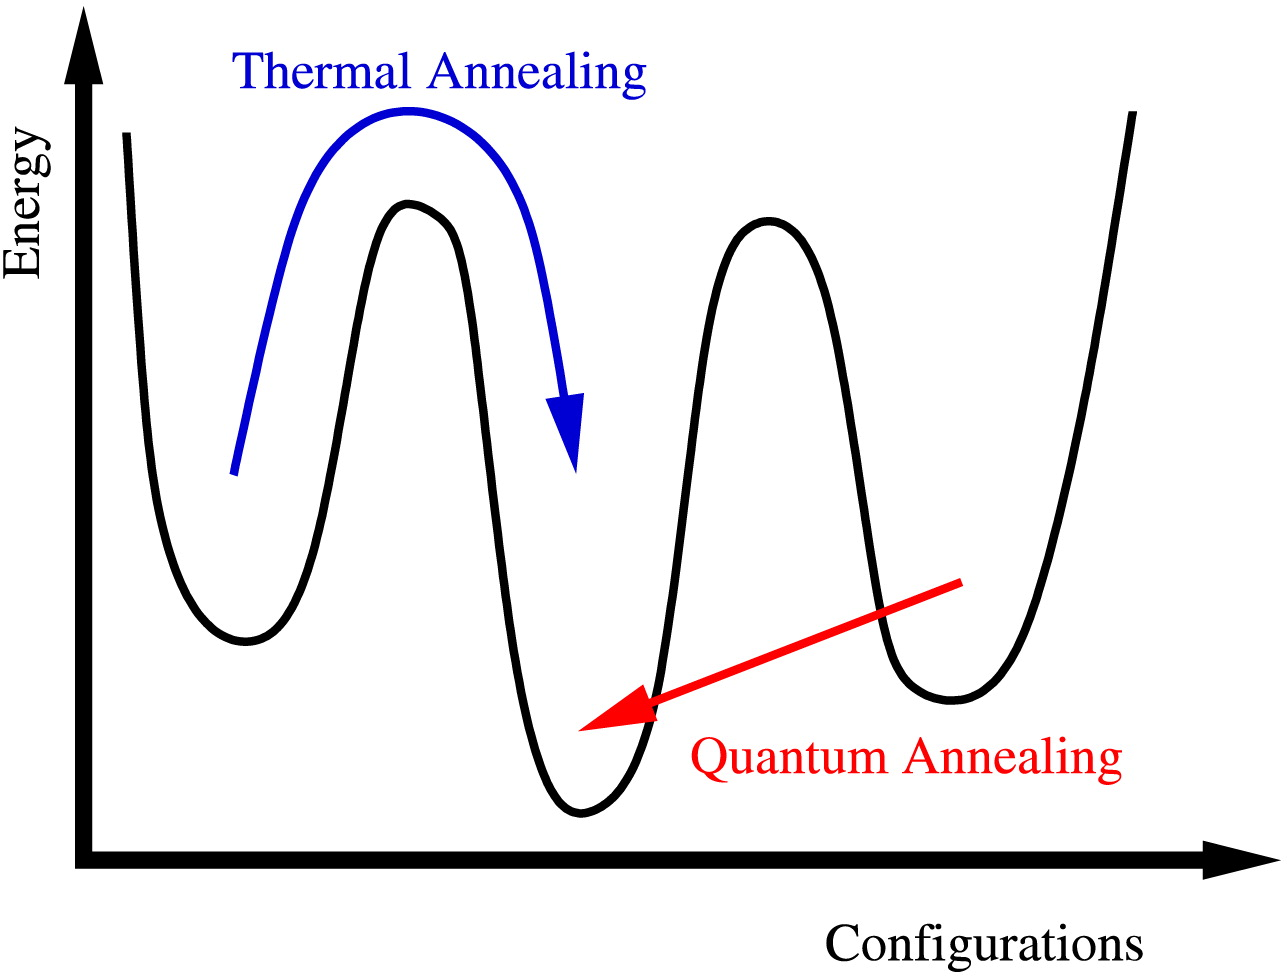
\includegraphics[width = 5cm]{Plots/tunneling.jpg}
      \hspace*{12pt}\hbox{\scriptsize {\footnotesize\itshape \href{https://doi.org/10.1016/j.physrep.2012.10.002}{V. Bapst et al., \textit{Physics Reports} 523 (2013)}}}
    \end{textblock*}
    \item transversales Ising Modell $H (t) = \underbrace{- \sum_{ij} J_{ij} \sigma_i^z \sigma_j^z - h \sum_i \sigma_i^z }_{H_0} \underbrace{- \Gamma (t) \sum_i \sigma_i^x}_{H_x(t)}  $ 
    \item $H_x (t)$ verursacht Tunneln zwischen Eigenzuständen von $H_0$
    \begin{itemize}
      \item schnellere Konvergenz
    \end{itemize}
    \item $\ket{\Psi(t)}$ durch Schrödingergleichung $i\frac{\partial \ket{\Psi(t)}}{\partial t} = H(t) \ket{\Psi(t)}$  \\ festgelegt
    \item wähle monoton fallende Funktionen für $\Gamma(t)$ (\enquote{ausglühen})
  \end{itemize} 
  \vspace*{1cm}
  \begin{block}{Adiabatisches Theorem der Quantenmechanik}
    \begin{center}
     System bleibt im selben Eigenzustand von $H$, wenn sich $H$ hinreichend langsam ändert  
    \end{center}    
  \end{block}

\end{frame}  

\begin{frame}{Adiabatische Zeit}
   \begin{itemize}
    \item minimale Zeit, damit sich System adiabatisch ändert $\tau$
    \item $\symup{\Delta} (s) = E_1 (s) - E_0 (s)$
    \item mindestens $\tau \propto \frac{1}{\symup{\Delta} (s)^2}$, schlimmstenfalls $\tau \propto \frac{1}{\symup{\Delta} (s)^3}$
    \item Problem: $\symup{\Delta} (s)$ sehr klein
    \begin{itemize}
      \item[\textrightarrow] $\tau \to \infty$
    \end{itemize}
   \end{itemize}
   \begin{textblock*}{5cm}(8cm, 4cm) % {block width} (coords)
    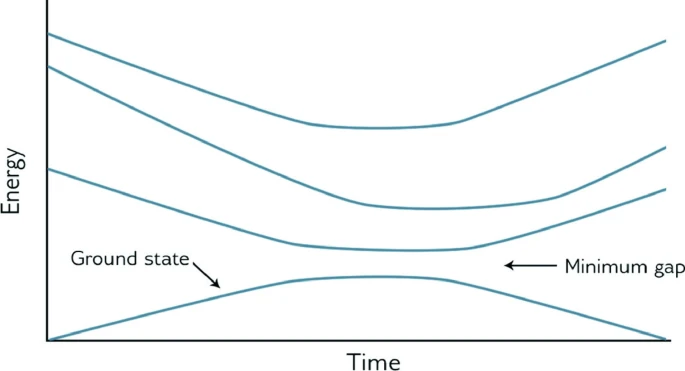
\includegraphics[width = 6.5cm]{Plots/gap.png}
    \hspace*{12pt}\hbox{\scriptsize {\footnotesize\itshape \href{https://link.springer.com/chapter/10.1007/978-3-031-13909-3_14}{E. R. Miranda (Ed.), Quantum Computer Music (2022)}}}
  \end{textblock*}

\end{frame}

\begin{frame}{Simulation zu simulated und quantum annealing}
  \begin{itemize}
    \item $P_\text{SA}(t)$: Wahrscheinlichkeit System in GZ zu finden
    \item $P_\text{QA}(t)$ = $|\braket{g}{\Psi(t)}|^2$: Wahrscheinlichkeit System in GZ $\ket{g}$ von $H_0$ zu finden
    \item $P_\text{SA}^{\text{st}}(T)$: Boltzmann-Faktor des GZ von $H_0$
    \item $P_\text{QA}^{\text{st}}(\Gamma) = | \braket{g}{\Psi_{\Gamma}} |^2$ mit $\ket{\Psi_{\Gamma}}$ als GZ von $H$
    \item $\lim_{t \to 0} \Gamma(t) = \lim_{t \to 0} T(t) = \infty$ bzw. $\lim_{t \to -\infty} \Gamma(t) = \lim_{t \to -\infty} T(t) = \infty$
    \begin{itemize}
      \item[\textrightarrow] Superposition aller Zustände gleicher Amplitude (QA)
      \item[\textrightarrow] Alle Zustände gleich wahrscheinlich (SA) 
    \end{itemize}
    \item Idealfall (adiabatisch): $\lim_{t \to \infty} P_{QA}(t) = \lim_{t \to \infty} P_{SA}(t) = 1$
    \begin{itemize}
      \item[\textrightarrow] Grundzustand gefunden
      \item[\textrightarrow] sonst: In einem lokalen Minimum \enquote{hängen} geblieben
    \end{itemize}
    \item 8 Spins 
  \end{itemize}
  \begin{textblock*}{5cm}(10cm, 4cm) % {block width} (coords)
    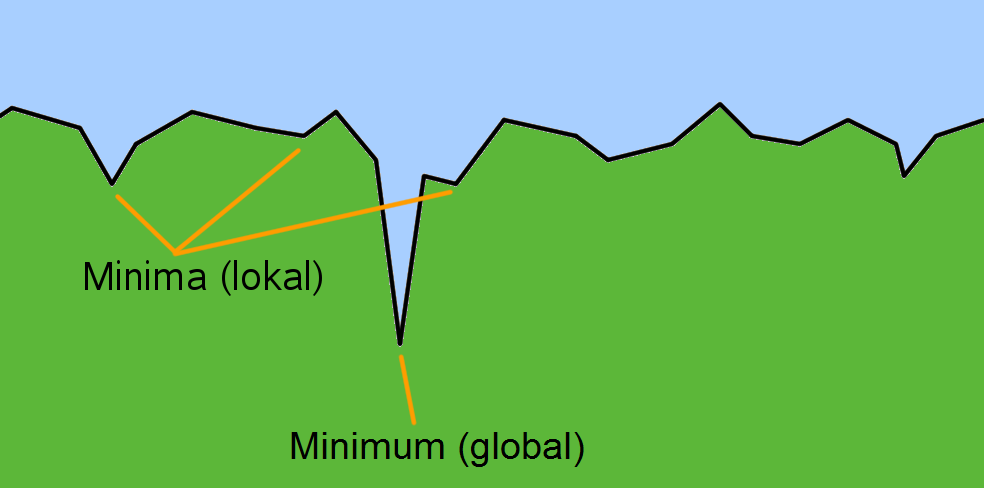
\includegraphics[width = 5.2cm]{Plots/SimAnnealingLandschaft.png}
    \hspace*{12pt}\hbox{\scriptsize {\footnotesize\itshape \href{https://de.wikipedia.org/wiki/Simulated_Annealing}{K. Fleischer, wikipedia.org}}}
  \end{textblock*}
  \begin{textblock*}{5cm}(0.5cm, 9cm)
    {\footnotesize \href{https://arxiv.org/abs/cond-mat/9804280}{Kadowaki, T, Nishimori, H, \textit{PHYSICAL REVIEW E } 1998}}
  \end{textblock*}
    
\end{frame}

\begin{frame}{Ergebnisse zu simulated und quantum annealing}
  \vspace*{-0.5cm}
  \begin{itemize}
    \item $P_\text{SA}(t)$: Wahrscheinlichkeit System in GZ zu finden
    \item $P_\text{QA}(t)$ = $|\braket{g}{\Psi(t)}|^2$: Wahrscheinlichkeit System in GZ $\ket{g}$ von $H_0$ zu finden
    \item $P_\text{SA}^{\text{st}}(T)$: Boltzmann-Faktor des GZ von $H_0$
    \item $P_\text{QA}^{\text{st}}(\Gamma) = | \braket{g}{\Psi_{\Gamma}} |^2$ mit $\ket{\Psi_{\Gamma}}$ als GZ von $H$
  \end{itemize}
  \vspace{1.5cm}
  \hspace{2cm}
  \fbox{\parbox{0.15 \textwidth}{
  \begin{itemize}
  \item $J_{ij}  = const$
  \item $h = 0.1$
  \end{itemize}}}
  \begin{textblock*}{7.5cm}(7.7cm, 3.5cm) % {block width} (coords)
  \begin{center}
    {\color{tugreen}
    $\Gamma(t) = T(t) = 3/ln(t+1)$ }
  \end{center}
    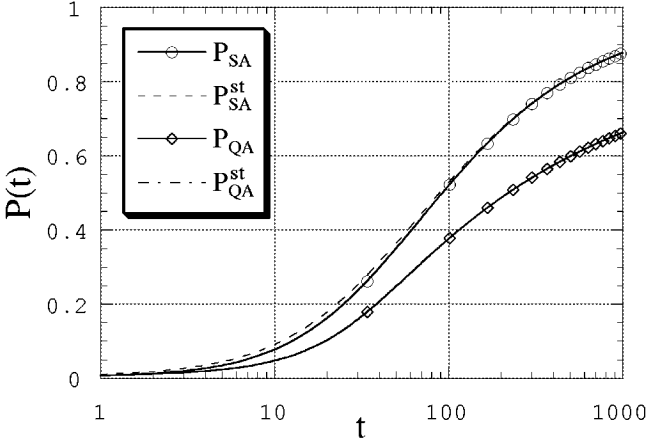
\includegraphics[width = 7.5cm]{Plots/ln.png}
    \end{textblock*}
    \begin{textblock*}{5cm}(0.5cm, 9cm)
      {\footnotesize \href{https://arxiv.org/abs/cond-mat/9804280}{Kadowaki, T, Nishimori, H, \textit{PHYSICAL REVIEW E } 1998}}
    \end{textblock*}
\end{frame}

\begin{frame}{Ergebnisse zu simulated und quantum annealing}
  \vspace*{-0.5cm}
  \begin{itemize}
    \item $P_\text{SA}(t)$: Wahrscheinlichkeit System in GZ zu finden
    \item $P_\text{QA}(t)$ = $|\braket{g}{\Psi(t)}|^2$: Wahrscheinlichkeit System in GZ $\ket{g}$ von $H_0$ zu finden
    \item $P_\text{SA}^{\text{st}}(T)$: Boltzmann-Faktor des GZ von $H_0$
    \item $P_\text{QA}^{\text{st}}(\Gamma) = | \braket{g}{\Psi_{\Gamma}} |^2$ mit $\ket{\Psi_{\Gamma}}$ als GZ von $H$
  \end{itemize}
  \vspace{1.5cm}
  \hspace{2cm}
  \fbox{\parbox{0.15 \textwidth}{
  \begin{itemize}
  \item $J_{ij}  = const$
  \item $h = 0.1$
  \end{itemize}}}
  \begin{textblock*}{7.5cm}(7.7cm, 3.5cm) % {block width} (coords)
    \begin{center}
      {\color{tugreen}
      $\Gamma(t) = T(t) = 3/\sqrt{t}$}
    \end{center}
    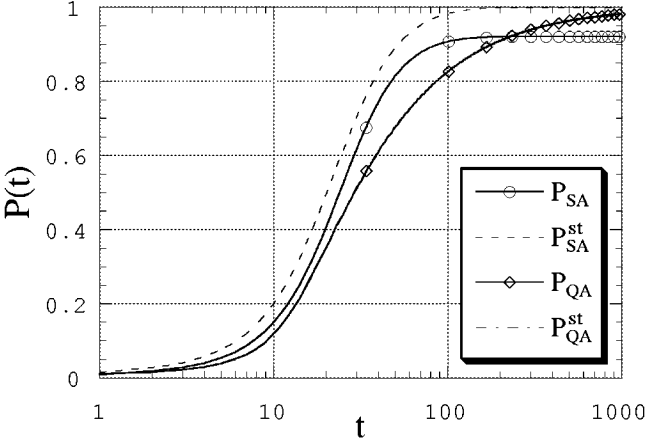
\includegraphics[width = 7.5cm]{Plots/sqrt.png}
  \end{textblock*}
  \begin{textblock*}{5cm}(0.5cm, 9cm)
    {\footnotesize \href{https://arxiv.org/abs/cond-mat/9804280}{Kadowaki, T, Nishimori, H, \textit{PHYSICAL REVIEW E } 1998}}
  \end{textblock*}
\end{frame}

\begin{frame}{Ergebnisse zu simulated und quantum annealing}
  \vspace*{-0.5cm}
  \begin{itemize}
    \item $P_\text{SA}(t)$: Wahrscheinlichkeit System in GZ zu finden
    \item $P_\text{QA}(t)$ = $|\braket{g}{\Psi(t)}|^2$: Wahrscheinlichkeit System in GZ $\ket{g}$ von $H_0$ zu finden
    \item $P_\text{SA}^{\text{st}}(T)$: Boltzmann-Faktor des GZ von $H_0$
    \item $P_\text{QA}^{\text{st}}(\Gamma) = | \braket{g}{\Psi_{\Gamma}} |^2$ mit $\ket{\Psi_{\Gamma}}$ als GZ von $H$
  \end{itemize}
  \vspace{1.5cm}
  \hspace{2cm}
  \fbox{\parbox{0.15 \textwidth}{
  \begin{itemize}
  \item $J_{ij}  = const$
  \item $h = 0.1$
  \end{itemize}}}
  \begin{textblock*}{7.5cm}(7.7cm, 3.5cm) % {block width} (coords)
    \begin{center}
      {\color{tugreen}
    $\Gamma(t) = T(t) = 3/t$}
  \end{center}
    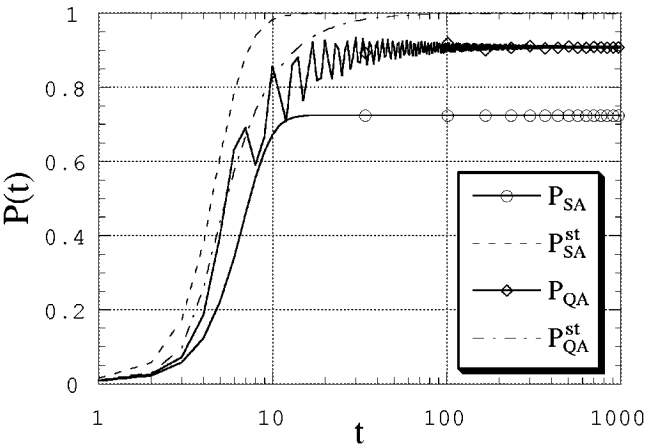
\includegraphics[width = 7.5cm]{Plots/t.png}
  \end{textblock*}
  \begin{textblock*}{5cm}(0.5cm, 9cm)
    {\footnotesize \href{https://arxiv.org/abs/cond-mat/9804280}{Kadowaki, T, Nishimori, H, \textit{PHYSICAL REVIEW E } 1998}}
  \end{textblock*}
\end{frame}

\section{Quadratic unconstrained binary optimization}

\begin{frame}{Binäre Variable}
  \begin{itemize}
    \item $x \in \{0,1\}$
    \item Beispiel: Aufenthaltsort von einem Truck
    \item Formulierung als Graph mit $N$ Knoten $i$
    \begin{itemize}
      \item ordne jedem Knoten $i$ eine binäre Varibale zu
      \item jedem Truck kann ein Vektor $x^j = (x^j_1, \ldots, x^j_N)$ von binären Variablen zugeordnet werden
    \end{itemize}
    \item Truck $j$ an Knoten $i$ \textrightarrow $x^j_i = 1$ sonst $x^j_k = 0$
  \end{itemize} 
\end{frame}

\begin{frame}{Binäre Variable}
  \begin{columns}
    \column{0.7 \textwidth}
      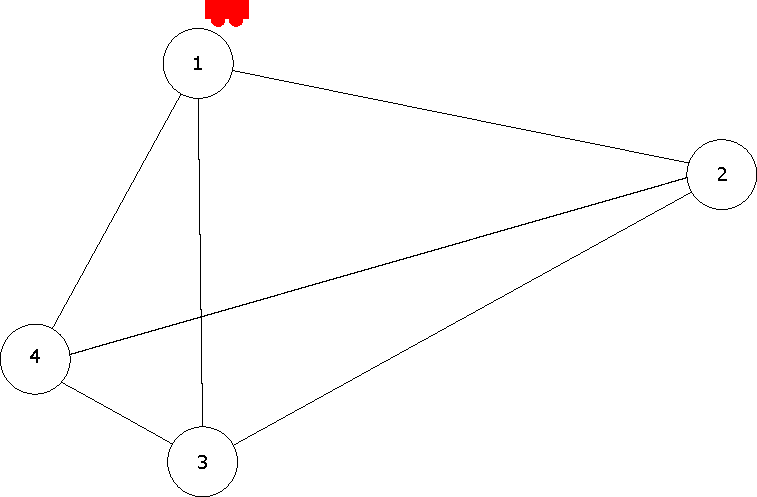
\includegraphics[width = \textwidth]{Plots/binary_1.pdf}
    \column{0.3 \textwidth}
  \begin{myequation}
    \underline{x}^\text{rot} \; \; = 
    \begin{pmatrix}
      1 \\ 0 \\ 0 \\ 0
    \end{pmatrix}
  \end{myequation}
  \end{columns}
\end{frame}

\begin{frame}{Binäre Variable}
  \begin{columns}
    \column{0.7 \textwidth}
      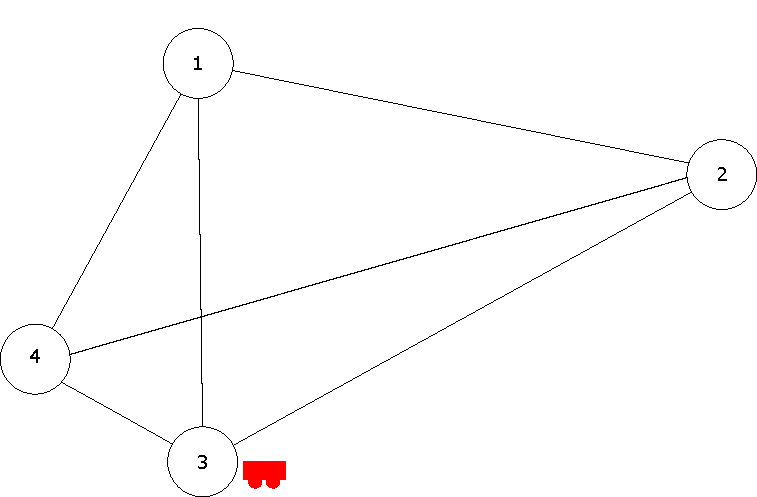
\includegraphics[width = \textwidth]{Plots/binary_2.pdf}
    \column{0.3 \textwidth}
  \begin{myequation}
    \underline{x}^\text{rot} \; \; = 
    \begin{pmatrix}
      0 \\ 0 \\ 1 \\ 0
    \end{pmatrix}
  \end{myequation}
  \end{columns}
\end{frame}

\begin{frame}{Binäre Variable}
  \begin{columns}
    \column{0.7 \textwidth}
      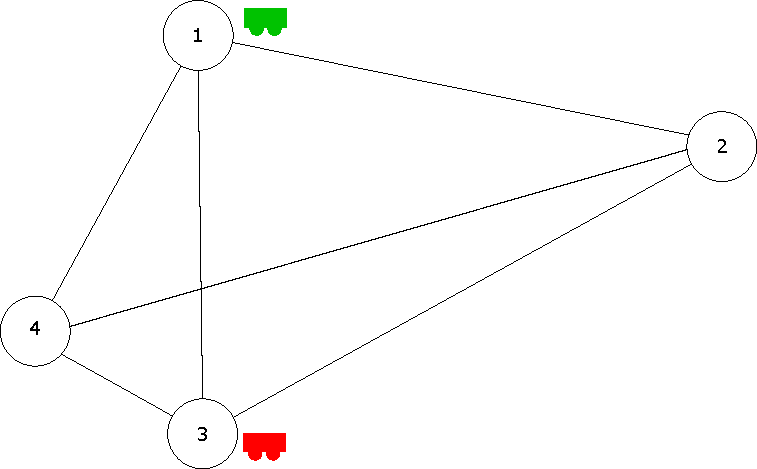
\includegraphics[width = \textwidth]{Plots/binary_3.pdf}
    \column{0.3 \textwidth}
  \begin{myequation}
    \underline{x}^\text{rot} \; \;  = 
    \begin{pmatrix}
      0 \\ 0 \\ 1 \\ 0
    \end{pmatrix}
  \end{myequation}
  \begin{myequation}
    \underline{x}^\text{grün} = 
    \begin{pmatrix}
      1 \\ 0 \\ 0 \\ 0
    \end{pmatrix}
  \end{myequation}
  \end{columns}
\end{frame}

\begin{frame}{Binäre Variable}
  \begin{columns}
    \column{0.7 \textwidth}
      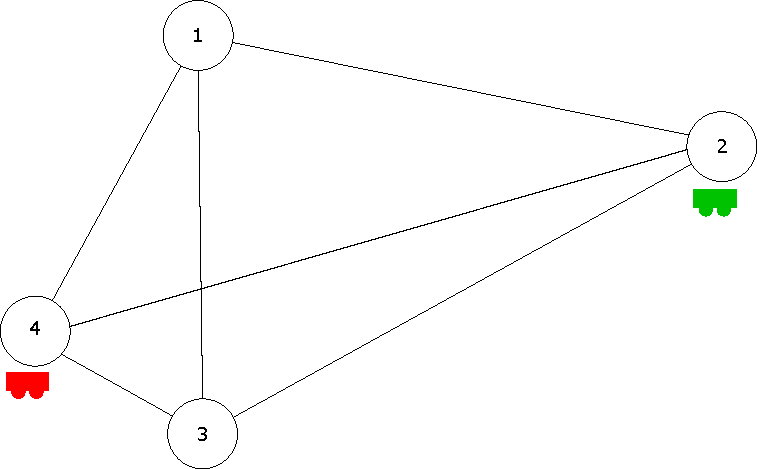
\includegraphics[width =  \textwidth]{Plots/binary_4.pdf}
    \column{0.3 \textwidth}
  \begin{myequation}
    \underline{x}^\text{rot} \; \;  = 
    \begin{pmatrix}
      0 \\ 0 \\ 0 \\ 1
    \end{pmatrix}
  \end{myequation}
  \begin{myequation}
    \underline{x}^\text{grün} = 
    \begin{pmatrix}
      0 \\ 1 \\ 0 \\ 0
    \end{pmatrix}
  \end{myequation}
  \end{columns}
\end{frame}

\begin{frame}{Quadratic unconstrained binary optimization (QUBO)}
  \begin{block}{Aufgabe}
    \center
     Minimiere $ f(\underline{x}, \underline{\underline{Q}}) = \sum_{ij} Q_{ij} x_ix_j$
  \end{block}
  \begin{itemize}
    \item $x_i \in \{0,1\}$ als binäre Variable
    \begin{itemize}
      \item lässt sich mittels $s_i = 2x_i - 1 \in \{-1, 1\}$ auf Ising-Variablen (\enquote{spin}) transformieren
    \end{itemize}
    \item $Q_{ij}$ definiert Wechselwirkung zwischen $x_i$
    \begin{itemize}
      \item allg. hermitesch (symmetrisch im Ising-Modell)
    \end{itemize}
  \end{itemize}
\end{frame}

\begin{frame}{Quadratic unconstrained binary optimization constrains}
  \begin{itemize}
    \item constraints lassen sich nicht direkt in der Hardware implementieren
    \begin{itemize}
      \item constraints als \enquote{Strafe} in der Kostenfunktion implementieren
    \end{itemize}
    \item Beispiel: Ein Truck darf sich nur an einem Punkt aufhalten
    \begin{itemize}
      \item $\sum_{i} x_i = 1 \iff \sum_i x_i - 1 = 0$
      \item in QUBO Problem umwandeln \textrightarrow $g(x_i) = (\sum_i x_i - 1)^2 $
      \item[\textrightarrow] $f \to f + \lambda g$
      \item constraint verletzt \textrightarrow Kostenfunktion erhöht
    \end{itemize}
    \item Lagrangeparameter $\lambda$ sehr groß wählen, damit constraint eingehalten
  \end{itemize}
\end{frame}

\section{Hardware embedding}

\begin{frame}{Quantum annealer von D-Wave Systems}
  \begin{itemize}
    \item D-Wave Systems als Hersteller von quantum annealer
    \item Qantum Processing Unit (QPU) mit QUBITs und couplern
    \begin{itemize}
      \item QUBITs und coupler sind gewichtet 
    \end{itemize}
    \item neuste Version: 5000 QUBITs mit 15 couplern pro QUBIT
    \item Nach annealing-Prozess die QUBIts auslesen
    \begin{itemize}
      \item[\textrightarrow] mögliches Energieminimum gefunden
    \end{itemize}
  \end{itemize}
  \vspace*{1cm}
  Unterschied zu Quantencomputer
    \begin{itemize}
      \item Quantum annealer nur für kombinatorische Optimierungsprobleme
      \item Quantencomputer nutzen Quantengatter (unitäre Operationen)
      \begin{itemize}
        \item kann mehr Problem lösen
      \end{itemize}
    \end{itemize}
  \begin{textblock*}{5cm}(11cm, 2cm) % {block width} (coords)
    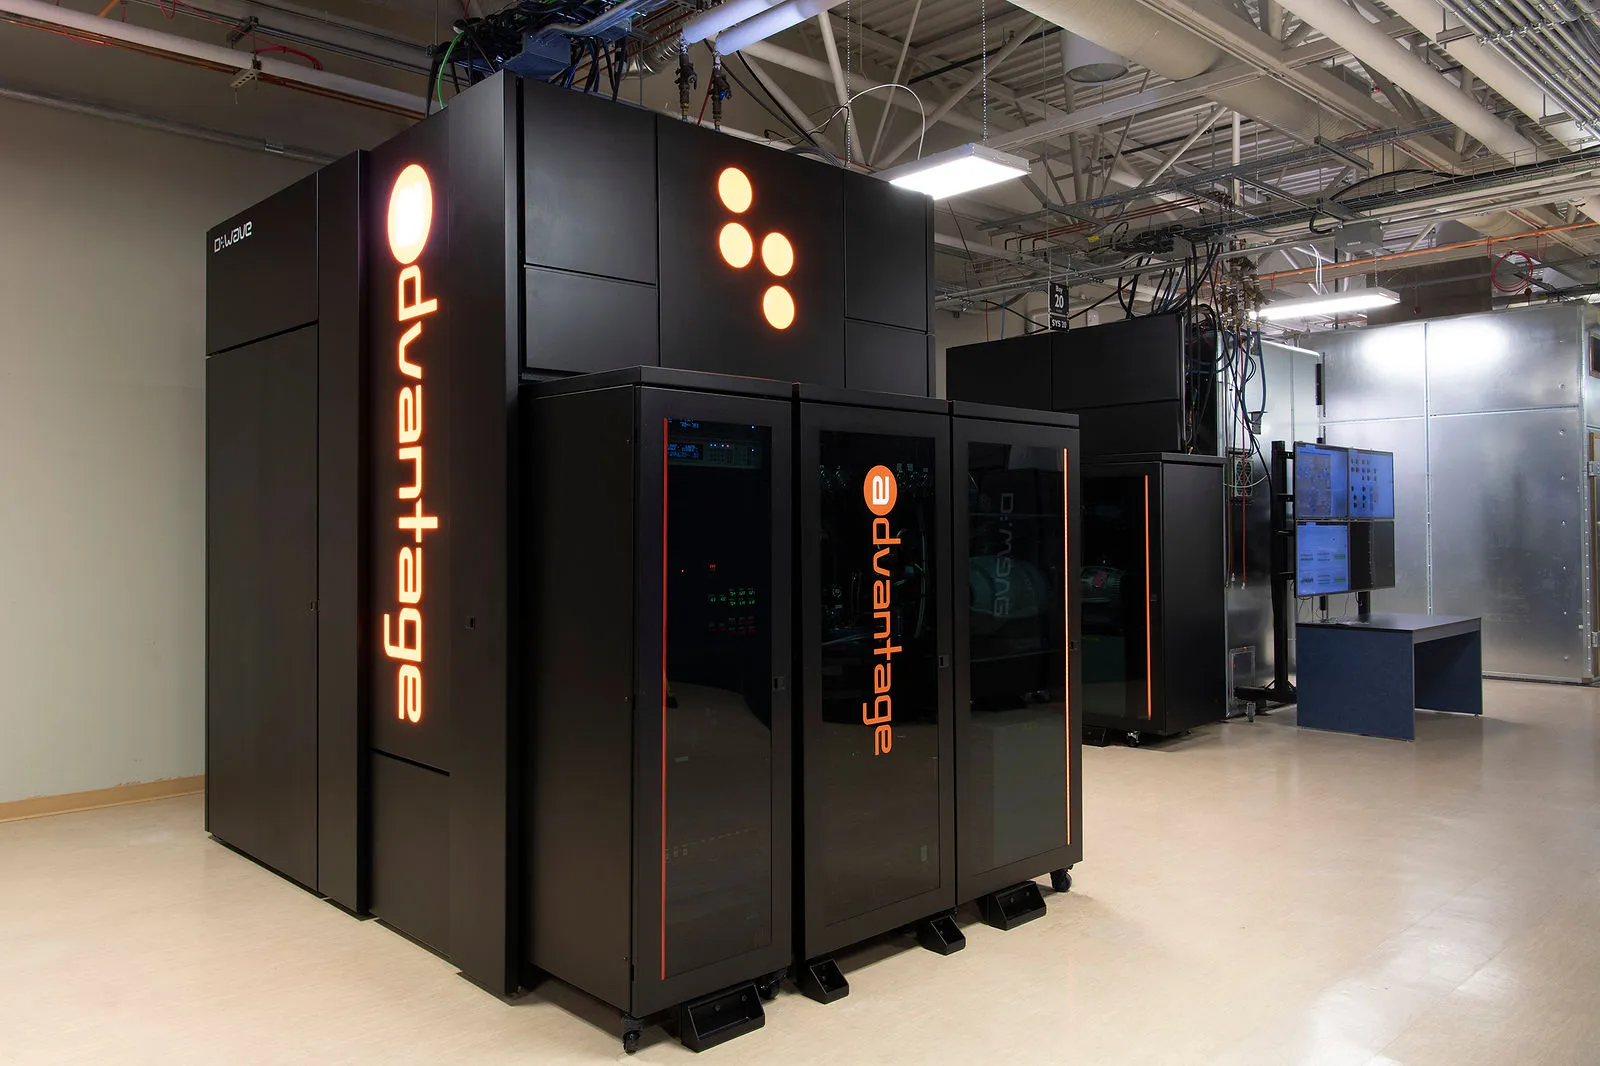
\includegraphics[width = 4.5cm]{Plots/advantage.png}
    \hspace*{12pt}\hbox{\scriptsize {\footnotesize\itshape \href{https://techcrunch.com/2020/09/29/d-wave-launches-its-5000-qubit-advantage-system/?guccounter=1&guce_referrer=aHR0cHM6Ly93d3cuZ29vZ2xlLmNvbS8&guce_referrer_sig=AQAAABB4SLnDOFLkzRsw3QLBP_BiwlTIN9jcs7feoLJi2DljlJifaHVtboTJQonfs2ulmdbT5fTNEU2jmeVP5gqNb_JTbAo88uHq76dEKRkeHYKpmXgEykCXVF3Y_-0ElGKOQqpS-rDrEZJWjMQh3x6OqCY4Pqpfeir7y8_RZCm6FRIW}{techchrunch.com}}}
  \end{textblock*}
  \begin{textblock*}{3cm}(12cm,5.8cm) % {block width} (coords)
    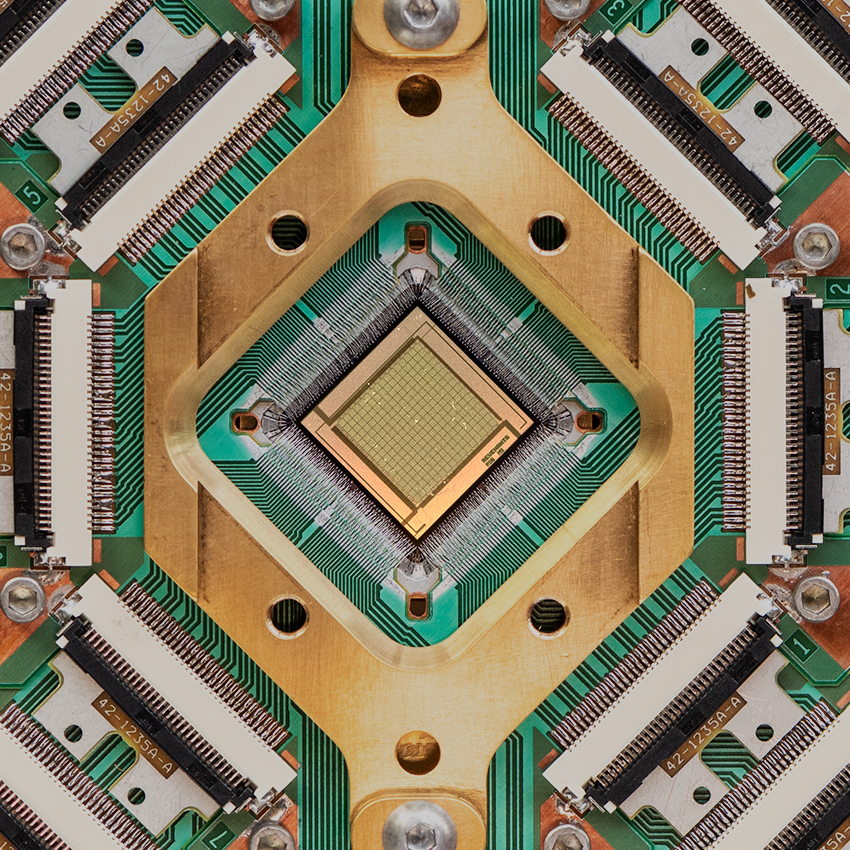
\includegraphics[width = 3cm]{Plots/QPU.jpg}
    \hspace*{12pt}\hbox{\scriptsize {\footnotesize\itshape \href{https://www.dwavesys.com/solutions-and-products/systems/}{dwavesys.com}}}
  \end{textblock*}  
\end{frame}

\begin{frame}{Embedding}
  \begin{itemize}
    \item D-Wave's QPU kann als Graph $U$ gesehen werden
    \begin{itemize}
      \item Gewichtete Vertices (QUBIT) $i \in V(U)$ 
      \item Gewichtete Kanten (coupler) $ij \in E(U)$
    \end{itemize}
    \item Gewichte:
    \begin{itemize}
      \item $h_i (t)$ \enquote{QUBIT bias}
      \item $\symup{\Delta}_i(t)$ \enquote{tunneling amplitude}
      \item $J_{ij}(t)$ \enquote{coupler strength}
    \end{itemize}
    \item formuliere transversalen Ising-Hamiltonian auf Graph $G$
    \item $H(t) = \sum_{i \in V(G)} h_i(t) \sigma_i^z + \sum_{ij \in E(G)} J_{ij}(t) \sigma_i^z \sigma_j^z + \sum_{i \in V(G)} \Delta_i (t) \sigma_i^x$
    \item Eigenergie des Ising-Hamiltonians $\epsilon(s_1, \ldots, s_n) = \sum_{i \in V(G)} h_i s_i + \sum_{ij \in E(G)} J_{ij} s_i s_j$
    \begin{itemize}
      \item spins $s_i \in \{-1,1\}$
    \end{itemize}
    \item Suche nach Grundzustandsenergie ist das \enquote{Ising Problem}
  \end{itemize}
  \begin{textblock*}{5cm}(10.4cm, 3cm) % {block width} (coords)
    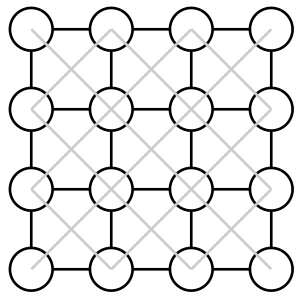
\includegraphics[width = 4.5cm]{Plots/4x4_graph.png}
    \hspace*{12pt}\hbox{\scriptsize {\footnotesize\itshape \href{https://doi.org/10.1016/j.physrep.2012.10.002}{V. Choi, \textit{D-Wave Systems Inc.} (2008)}}}
  \end{textblock*}  
\end{frame}

\begin{frame}{Embedding}
  \begin{textblock*}{5cm}(10cm, 1.9cm) % {block width} (coords)
    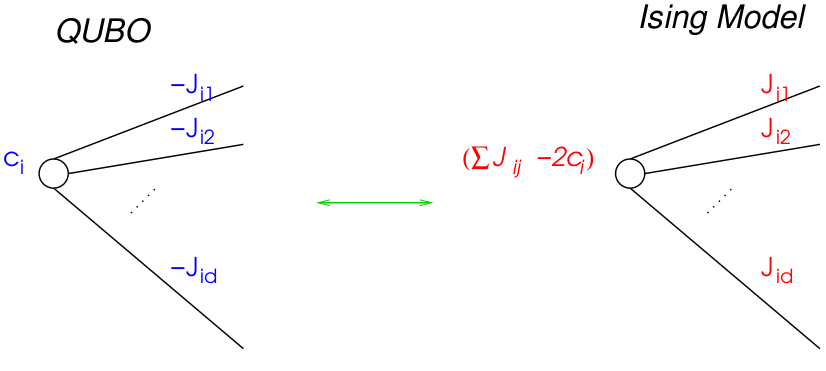
\includegraphics[width = 5.5cm]{Plots/qubo_ising.png}
    \hspace*{12pt}\hbox{\scriptsize {\footnotesize\itshape \href{https://doi.org/10.1016/j.physrep.2012.10.002}{V. Choi, \textit{D-Wave Systems Inc.} (2008)}}}
  \end{textblock*}
   \begin{itemize}
    \item Ising Problem äquivalent zu QUBO Problem auf dem selben Graph $G$
    \begin{itemize}
      \item $Y(x_1, \ldots, x_n) = \sum_{i \in V(G)} c_i x_i - \sum_{ij \in E(G)} J_{ij} x_i x_j $ maximieren
      \item $x_i \in \{0,1\}$ 
    \end{itemize}
  \end{itemize}
    \begin{block}{Ziel}
       $G$ in $U$ einbetten (\enquote{subgraph-embedding}) und somit das Ising/QUBO Problem lösen 
    \end{block}
    \begin{itemize}
      \item Problem: Einschränkungen auf $U$ (z.B. Anzahl der coupler) übertragen sich auf $G$
      \begin{itemize}
        \item[\textrightarrow] \enquote{dummy}-Vertices mit ferromagnetischer Kopplung einführen
      \end{itemize}
    \end{itemize}
\end{frame}

\begin{frame}{Minor embedding}
  \vspace*{1cm}
  \begin{itemize}
  \item logischer QUBIT $i$ aus $G$ wird auf subtree $T_i$ physischer QUBITs aus $G_\text{emb} \subset U$ abgebildet
  \item ferromagnetische Kopplung zwischen \enquote{dummy}-Vertices muss hinreichend groß sein
  \end{itemize}
  \vspace*{1cm}
  \begin{varblock}[6cm]{Ziel}
    Parameter des minor-embedding auf ursprüngliche Ising/QUBO Variablen zurückführen
  \end{varblock}
  \vspace*{4cm}
  \begin{textblock*}{6cm}(8.5cm, 4.5cm) % {block width} (coords)
    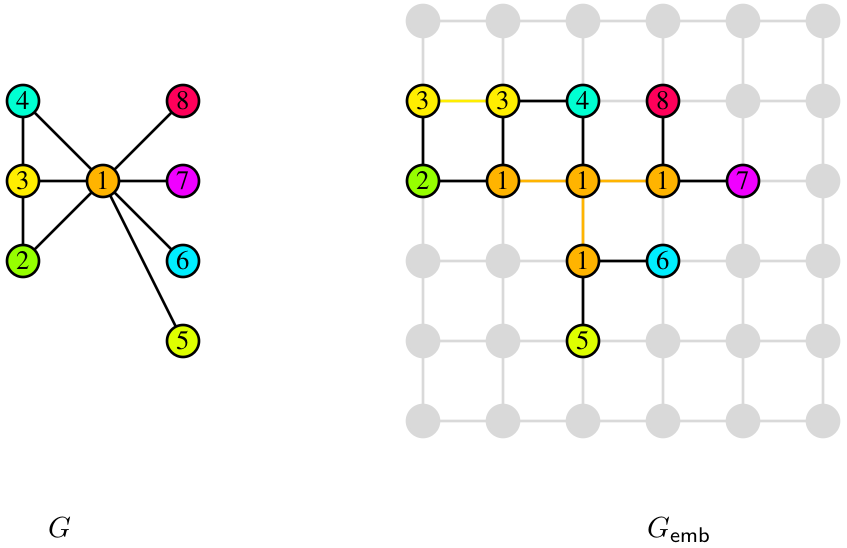
\includegraphics[width = 6.5cm]{Plots/G_emb.png}
    \hspace*{12pt}\hbox{\scriptsize {\footnotesize\itshape \href{https://doi.org/10.1016/j.physrep.2012.10.002}{V. Choi, \textit{D-Wave Systems Inc.} (2008)}}}
  \end{textblock*}
\end{frame}

\begin{frame}{Minor embedding}
  \begin{itemize}
    \item $\epsilon^\text{emb}(s_1, \ldots, s_N) = \sum_{i \in V(G_\text{emb})} h_i's_i + \sum_{ij \in E(G_\text{emb})} J_{ij}' s_i s_j $ minimieren
    \item $\tau : V(G) \times V(G) \to V(U)$, so dass $i_{\tau (i,j)} \in V(T_i), \; j_{\tau (j,i)} \in V(T_j)$ mit $i_{\tau (i,j)} j_{\tau (j,i)} \in E(U)$
    \item $\text{OE}(G_\text{emb}) = \cup_{ij \in E(G)} i_{\tau (i,j)} j_{\tau (j,i)}$ sind ursprüngliche coupler 
    \begin{itemize}
      \item[\textrightarrow] $J_{i_{\tau (i,j)} j_{\tau (j,i)}}' = J_{ij}$ für $i_{\tau (i,j)} j_{\tau (j,i)} \in \text{OE}(G_\text{emb})$
    \end{itemize}
    \item ferromagnetische coupler strength $F_k^{ij}$ für $ij \in E(T_i)$
    \item bias $h_i$ der logischen QUBITs auf physische QUBITs verteilen 
    \begin{itemize}
      \item[\textrightarrow] $\sum_{i_k \in V(T_i)} h_{i_k}' = h_i$
    \end{itemize} 
  \end{itemize}
  \begin{block}{Finale Energie}
    \begin{equation*}
      \epsilon^{\text{emb}}(s_1, \ldots, s_N) = \sum_{i \in V(G)} \left (
        \sum_{i_k \in V(T_i)} h_{i_k}' s_{i_k} + \sum_{i_p i_q \in E(T_i)} F_i^{pq} s_{i_p} s_{i_q} \right ) 
        + \sum_{ij \in E(G)} J_{ij} s_{i_{\tau(ij)}} s_{j_{\tau(ij)}}
    \end{equation*}
  \end{block}
  \begin{textblock*}{6cm}(11cm, 1.7cm) % {block width} (coords)
    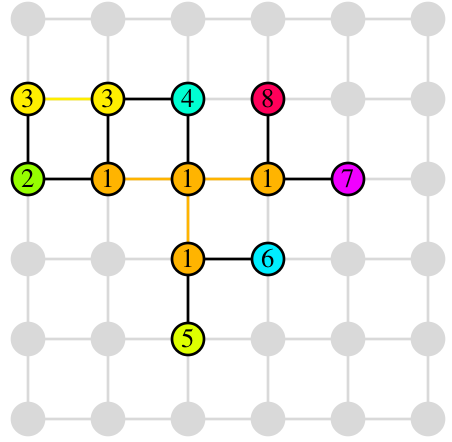
\includegraphics[width = 4cm]{Plots/graph_cut.png}
    \hspace*{12pt}\hbox{\scriptsize {\footnotesize\itshape \href{https://doi.org/10.1016/j.physrep.2012.10.002}{V. Choi, \textit{D-Wave Systems Inc.} (2008)}}}
  \end{textblock*}
\end{frame}

\section{Fallbeispiel Aisin Corporation}
\begin{frame}{Fallbeispiel Aisin Corporation}
  \begin{textblock*}{5cm}(11cm, 2cm) % {block width} (coords)
    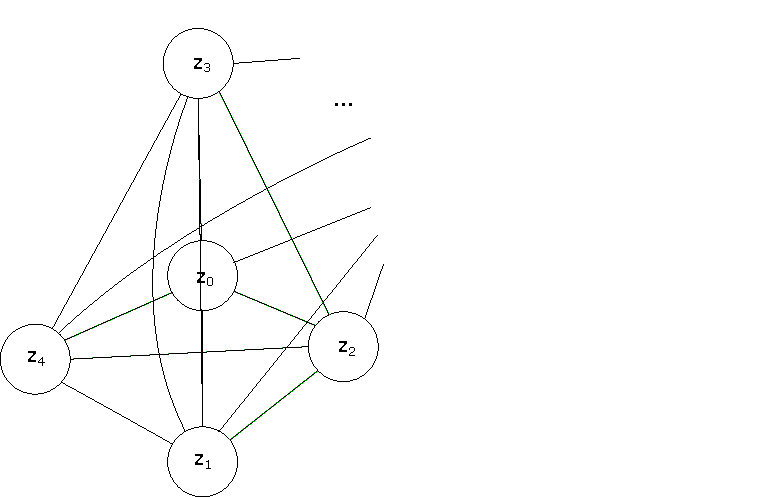
\includegraphics[width = 7cm]{Plots/ex.pdf}
  \end{textblock*}
  \begin{itemize}
    \item Zeit für Route $\xi$ : $\text{time}(\xi) = \sum_{t=1}^{k-1} T_{\xi_t, \xi_{t+1}}$
    \item off-board-demand $D_{ij}$, der von $i$ nach $j$ gebracht werden muss
  \end{itemize}
  Terme für QUBO-Formulierung:
  \begin{itemize}
    \item $f_\text{local} (\{ x_i \}) = A_\text{local} \sum_t \left ( 1-\sum_i x_{it} \right )^2$
    \item $f_\text{time} (\{ x_i \}) = A_\text{time} \sum_{ijt} T_{ij} x_{it}x_{jt+1}$
    \item $f_\text{demand} (\{ x_i \}) = - A_\text{demand} \sum_{ijt} \sum_{\delta = 1}^{\delta_*(t)} D_{ij} x_{it} x_{j t+\delta}$ mit $\delta_*(t) = \text{min}(\delta_\text{max}, \tau -1 -t)$
    \item $f_\text{nonredundant}^I (\{ x_i \}) = A_{\text{nonredundant}}\sum_{ij} I_{ij} \sum_{\delta = 2}^{\tau - 2} \sum_{t=0}^{\tau - 2 - \delta} x_{it} x_{j t+1} x_{i t+\delta} x_{j t+ 1 +\delta}$
    \begin{itemize}
      \item Vorsicht: Grad des Polynoms muss noch auf zwei reduziert werden
    \end{itemize}
    \vspace*{0.5cm}
    \begin{equation*}
      A_\text{local} = 5000, \quad A_\text{demand} = 320, \quad A_\text{time} = 0.01\quad A_\text{nonredundant} = 1  
    \end{equation*}
  \end{itemize}

  \begin{textblock*}{6cm}(0.5cm, 9cm)
    {\footnotesize \href{https://www.nature.com/articles/s41598-023-31765-8}{Weinberg, S.J., Sanches, F., Ide, T. et al. Sci Rep 13, 4770 (2023)}}
  \end{textblock*}

\end{frame}

\begin{frame}{Fallbeispiel Aisin Corporation}
  \begin{textblock*}{5cm}(0.5cm, 3cm) % {block width} (coords)
    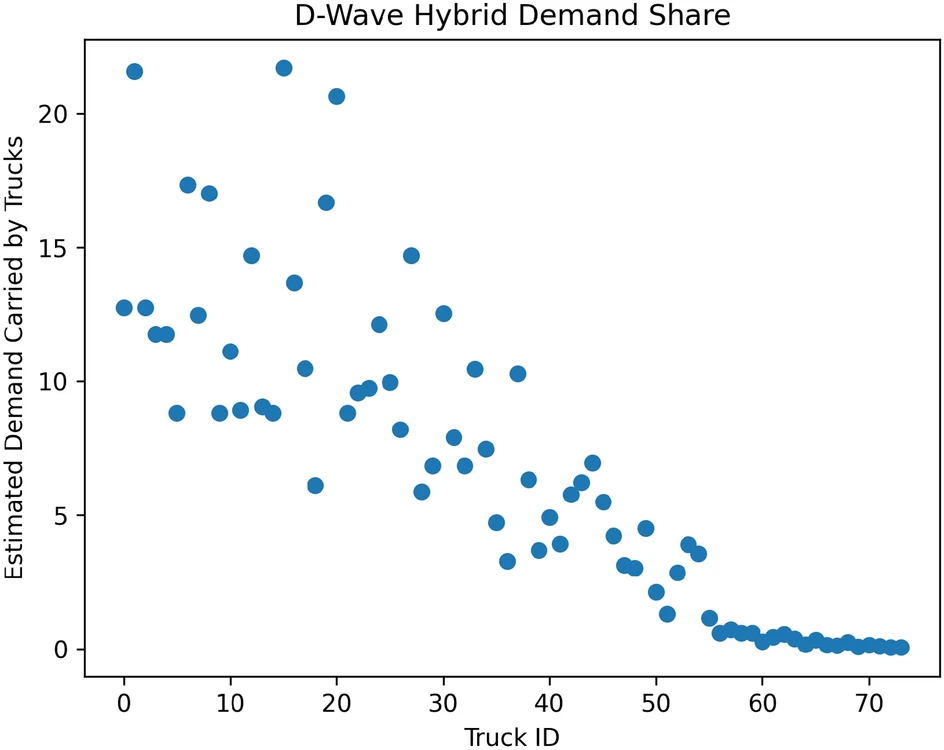
\includegraphics[width = 7cm]{Plots/74.png}
  \end{textblock*}
  \begin{textblock*}{5cm}(8.2cm, 3cm) % {block width} (coords)
    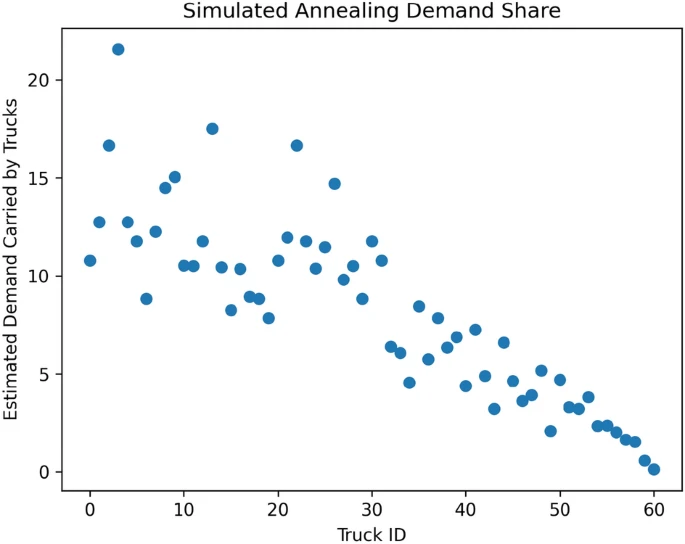
\includegraphics[width = 7cm]{Plots/61.png}
  \end{textblock*}
  \begin{textblock*}{6cm}(0.5cm, 9cm)
    {\footnotesize \href{https://www.nature.com/articles/s41598-023-31765-8}{Weinberg, S.J., Sanches, F., Ide, T. et al. Sci Rep 13, 4770 (2023)}}
  \end{textblock*}
\end{frame}

\begin{frame}{Fallbeispiel Aisin Corporation}
  \begin{textblock*}{5cm}(1cm, 2.5cm) % {block width} (coords)
    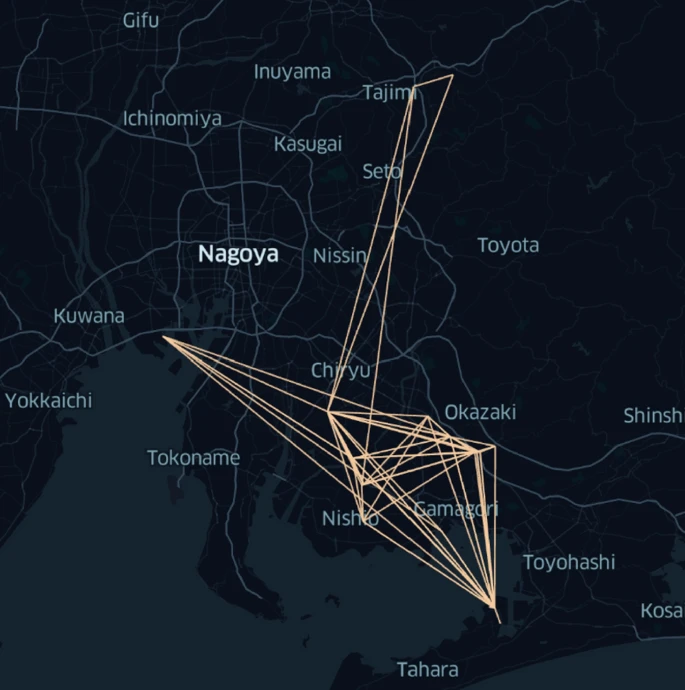
\includegraphics[width = 6cm]{Plots/before.png}
  \end{textblock*}
  \begin{textblock*}{5cm}(9cm, 2.5cm) % {block width} (coords)
    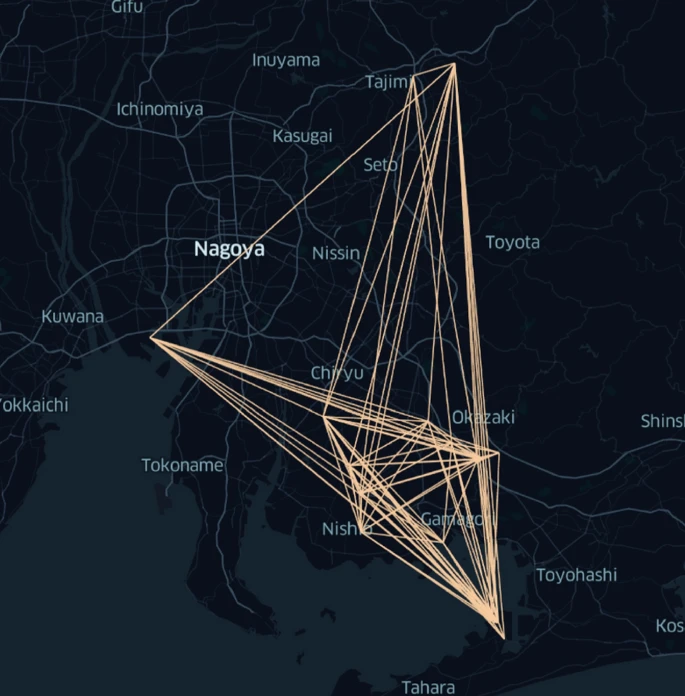
\includegraphics[width = 6cm]{Plots/after.png}
  \end{textblock*}
  \begin{textblock*}{6cm}(0.5cm, 9cm)
    {\footnotesize \href{https://www.nature.com/articles/s41598-023-31765-8}{Weinberg, S.J., Sanches, F., Ide, T. et al. Sci Rep 13, 4770 (2023)}}
  \end{textblock*}
\end{frame}

\section{Zusammenfassung und Ausblick}
\begin{frame}{Zusammenfassung und Ausblick}
\end{frame}

\begin{frame}{Quellen}
  \begin{itemize}
    \item Bapst, V. et al., The quantum adiabatic algorithm applied to random optimization
    problems: The quantum spin glass perspective, \textit{ScienceDirect} 523 (2013), https://doi.org/10.1016/j.physrep.2012.10.002
    \item Kadowaki, T. et al. Quantum annealing in the transverse Ising model,  \textit{PHYSICAL REVIEW E} 58 (1998), https://doi.org/10.48550/arXiv.cond-mat/9804280
    \item Rieffel, E.G., Venturelli, D., O’Gorman, B. et al. A case study in programming a quantum annealer for hard operational planning problems. Quantum Inf Process 14, 1–36 (2015). https://doi.org/10.1007/s11128-014-0892-x
    \item Choi, V. Minor-embedding in adiabatic quantum computation: I. The parameter setting problem. Quantum Inf Process 7, 193–209 (2008). https://doi.org/10.1007/s11128-008-0082-9
    \item Jain, S, Solving the Traveling Salesman
    Problem on the D-Wave Quantum
    Computer, \textit{
      Frontiers in Physics}, Volume 9, id.646 (2021)
 ,doi: 10.3389/fphy.2021.760783
    \item Sangwan, Shabnam. (2018). Literature Review on Travelling Salesman Problem. \textit{International Journal of Research.} 5. 1152. 
    \item Weinberg, S.J., Sanches, F., Ide, T. et al. Supply chain logistics with quantum and classical annealing algorithms. Sci Rep 13, 4770 (2023). https://doi.org/10.1038/s41598-023-31765-8
    \item Yarkoni, S et al., Quantum annealing for industry applications:
    introduction and review, \textit{IOP Publishing} 85-10 (2022), https://dx.doi.org/10.1088/1361-6633/ac8c54
  \end{itemize}
\end{frame}

\begin{frame}{Backup-Folien für Detailfragen}
  Details, evtl. Rechnungen und Zahlenwerte für Fragen
\end{frame}

\end{document}